\documentclass{article}
\usepackage{graphics} 
\usepackage{hyperref}
\usepackage{fixltx2e}
\usepackage{amssymb}
\usepackage{tikz}
\usepackage{amsmath}

\author{Kevin Zollicoffer}
\title{Data Mining in R\\Assignment 2}
\date{1/26/2013}

% no indents
\setlength\parindent{0pt}

\usepackage{Sweave}
\begin{document}
\maketitle
%\tableofcontents
\Sconcordance{concordance:KevinZollicoffer_Assignment2.tex:KevinZollicoffer_Assignment2.Rnw:%
1 15 1 1 0 29 1 1 2 1 0 1 1 19 0 1 2 1 1 1 2 4 0 1 2 1 1 1 2 4 0 1 2 2 %
1 1 7 9 0 1 2 1 7 9 0 1 2 1 1 1 5 1072 0 1 1 594 0 1 2 1 1 1 2 5 0 1 2 %
1 1 1 2 1 0 1 1 32 0 1 2 2 1 1 3 2 0 1 1 4 0 1 2 1 3 2 0 1 1 4 0 1 2 1 %
3 2 0 1 1 4 0 1 2}


\section*{Q.1}
The proportion of variance in the observations is almost completely (1) explained by the model. 

\section*{Q.2}
k-1 integer [0:1] variables used to represent categories of a categorical variable where k is the number of categories.

\section*{Q.3}
It will fit the training data too perfectly capturing spurious relationships of the training data set, thus performing badly when faced with a new data sample for which predictions are required. 

\section*{Q.4}
To avoid over-fitting

\section*{Q.5}
Calculating the performance metrics using the training data is unreliable because the obtained estimates are biased. The performance metrics would hardly generalize over new sampeles for which the target variable is unknown. 

\section*{Q.6}
Testing the model on data not used for it's consrtruction

\section*{Q.7}
The model is performing very poorly. NMSE values are usually between 0 and 1 with lower values indicating better model performance

\section*{Assignment}

First we load the data

\begin{Schunk}
\begin{Sinput}
> load("~/R/PASS/DMinR/AlgaeBlooms/algae.RData")
> head(algae)
\end{Sinput}
\begin{Soutput}
  season  size  speed mxPH mnO2     Cl    NO3     NH4    oPO4     PO4 Chla   a1
1 winter small medium 8.00  9.8 60.800  6.238 578.000 105.000 170.000 50.0  0.0
2 spring small medium 8.35  8.0 57.750  1.288 370.000 428.750 558.750  1.3  1.4
3 autumn small medium 8.10 11.4 40.020  5.330 346.667 125.667 187.057 15.6  3.3
4 spring small medium 8.07  4.8 77.364  2.302  98.182  61.182 138.700  1.4  3.1
5 autumn small medium 8.06  9.0 55.350 10.416 233.700  58.222  97.580 10.5  9.2
6 winter small   high 8.25 13.1 65.750  9.248 430.000  18.250  56.667 28.4 15.1
    a2   a3  a4   a5   a6  a7
1  0.0  0.0 0.0 34.2  8.3 0.0
2  7.6  4.8 1.9  6.7  0.0 2.1
3 53.6  1.9 0.0  0.0  0.0 9.7
4 41.0 18.9 0.0  1.4  0.0 1.4
5  2.9  7.5 0.0  7.5  4.1 1.0
6 14.6  1.4 0.0 22.5 12.6 2.9
\end{Soutput}
\end{Schunk}

Load the DMwR library
\begin{Schunk}
\begin{Sinput}
> library(DMwR)
\end{Sinput}
\end{Schunk}

Impute missing data
\begin{Schunk}
\begin{Sinput}
> clean.algae <- knnImputation(algae, k = 10)
\end{Sinput}
\end{Schunk}

Prepare cross validation functions

\begin{Schunk}
\begin{Sinput}
> cv.rpart <- function(form,train,test,...) {
+ m <- rpartXse(form,train,...)
+ p <- predict(m,test)
+ mae <- mean(abs(p-resp(form,test)))
+ c(mae=mae)
+ }
\end{Sinput}
\end{Schunk}

\begin{Schunk}
\begin{Sinput}
> DSs <- sapply(names(clean.algae)[12:18],
+ function(x,names.attrs) {
+ f <- as.formula(paste(x,"~ ."))
+ dataset(f,clean.algae[,c(names.attrs,x)],x)
+ },
+ names(clean.algae)[1:11])
\end{Sinput}
\end{Schunk}

Perform comparisons
\begin{Schunk}
\begin{Sinput}
> res.all <- experimentalComparison(
+ DSs,
+ c(variants('cv.rpart',se=c(0,0.2,0.4,0.6,0.8,1.0,1.2,1.4,1.6,1.8))),
+ cvSettings(5,2,1234))
\end{Sinput}
\begin{Soutput}
#####  CROSS VALIDATION  EXPERIMENTAL COMPARISON #####

** DATASET :: a1

++ LEARNER :: cv.rpart  variant ->  cv.rpart.v1 

 5 x 2 - Fold Cross Validation run with seed =  1234 
Repetition  1 
Fold:  1  2
Repetition  2 
Fold:  1  2
Repetition  3 
Fold:  1  2
Repetition  4 
Fold:  1  2
Repetition  5 
Fold:  1  2


++ LEARNER :: cv.rpart  variant ->  cv.rpart.v2 

 5 x 2 - Fold Cross Validation run with seed =  1234 
Repetition  1 
Fold:  1  2
Repetition  2 
Fold:  1  2
Repetition  3 
Fold:  1  2
Repetition  4 
Fold:  1  2
Repetition  5 
Fold:  1  2


++ LEARNER :: cv.rpart  variant ->  cv.rpart.v3 

 5 x 2 - Fold Cross Validation run with seed =  1234 
Repetition  1 
Fold:  1  2
Repetition  2 
Fold:  1  2
Repetition  3 
Fold:  1  2
Repetition  4 
Fold:  1  2
Repetition  5 
Fold:  1  2


++ LEARNER :: cv.rpart  variant ->  cv.rpart.v4 

 5 x 2 - Fold Cross Validation run with seed =  1234 
Repetition  1 
Fold:  1  2
Repetition  2 
Fold:  1  2
Repetition  3 
Fold:  1  2
Repetition  4 
Fold:  1  2
Repetition  5 
Fold:  1  2


++ LEARNER :: cv.rpart  variant ->  cv.rpart.v5 

 5 x 2 - Fold Cross Validation run with seed =  1234 
Repetition  1 
Fold:  1  2
Repetition  2 
Fold:  1  2
Repetition  3 
Fold:  1  2
Repetition  4 
Fold:  1  2
Repetition  5 
Fold:  1  2


++ LEARNER :: cv.rpart  variant ->  cv.rpart.v6 

 5 x 2 - Fold Cross Validation run with seed =  1234 
Repetition  1 
Fold:  1  2
Repetition  2 
Fold:  1  2
Repetition  3 
Fold:  1  2
Repetition  4 
Fold:  1  2
Repetition  5 
Fold:  1  2


++ LEARNER :: cv.rpart  variant ->  cv.rpart.v7 

 5 x 2 - Fold Cross Validation run with seed =  1234 
Repetition  1 
Fold:  1  2
Repetition  2 
Fold:  1  2
Repetition  3 
Fold:  1  2
Repetition  4 
Fold:  1  2
Repetition  5 
Fold:  1  2


++ LEARNER :: cv.rpart  variant ->  cv.rpart.v8 

 5 x 2 - Fold Cross Validation run with seed =  1234 
Repetition  1 
Fold:  1  2
Repetition  2 
Fold:  1  2
Repetition  3 
Fold:  1  2
Repetition  4 
Fold:  1  2
Repetition  5 
Fold:  1  2


++ LEARNER :: cv.rpart  variant ->  cv.rpart.v9 

 5 x 2 - Fold Cross Validation run with seed =  1234 
Repetition  1 
Fold:  1  2
Repetition  2 
Fold:  1  2
Repetition  3 
Fold:  1  2
Repetition  4 
Fold:  1  2
Repetition  5 
Fold:  1  2


++ LEARNER :: cv.rpart  variant ->  cv.rpart.v10 

 5 x 2 - Fold Cross Validation run with seed =  1234 
Repetition  1 
Fold:  1  2
Repetition  2 
Fold:  1  2
Repetition  3 
Fold:  1  2
Repetition  4 
Fold:  1  2
Repetition  5 
Fold:  1  2


** DATASET :: a2

++ LEARNER :: cv.rpart  variant ->  cv.rpart.v1 

 5 x 2 - Fold Cross Validation run with seed =  1234 
Repetition  1 
Fold:  1  2
Repetition  2 
Fold:  1  2
Repetition  3 
Fold:  1  2
Repetition  4 
Fold:  1  2
Repetition  5 
Fold:  1  2


++ LEARNER :: cv.rpart  variant ->  cv.rpart.v2 

 5 x 2 - Fold Cross Validation run with seed =  1234 
Repetition  1 
Fold:  1  2
Repetition  2 
Fold:  1  2
Repetition  3 
Fold:  1  2
Repetition  4 
Fold:  1  2
Repetition  5 
Fold:  1  2


++ LEARNER :: cv.rpart  variant ->  cv.rpart.v3 

 5 x 2 - Fold Cross Validation run with seed =  1234 
Repetition  1 
Fold:  1  2
Repetition  2 
Fold:  1  2
Repetition  3 
Fold:  1  2
Repetition  4 
Fold:  1  2
Repetition  5 
Fold:  1  2


++ LEARNER :: cv.rpart  variant ->  cv.rpart.v4 

 5 x 2 - Fold Cross Validation run with seed =  1234 
Repetition  1 
Fold:  1  2
Repetition  2 
Fold:  1  2
Repetition  3 
Fold:  1  2
Repetition  4 
Fold:  1  2
Repetition  5 
Fold:  1  2


++ LEARNER :: cv.rpart  variant ->  cv.rpart.v5 

 5 x 2 - Fold Cross Validation run with seed =  1234 
Repetition  1 
Fold:  1  2
Repetition  2 
Fold:  1  2
Repetition  3 
Fold:  1  2
Repetition  4 
Fold:  1  2
Repetition  5 
Fold:  1  2


++ LEARNER :: cv.rpart  variant ->  cv.rpart.v6 

 5 x 2 - Fold Cross Validation run with seed =  1234 
Repetition  1 
Fold:  1  2
Repetition  2 
Fold:  1  2
Repetition  3 
Fold:  1  2
Repetition  4 
Fold:  1  2
Repetition  5 
Fold:  1  2


++ LEARNER :: cv.rpart  variant ->  cv.rpart.v7 

 5 x 2 - Fold Cross Validation run with seed =  1234 
Repetition  1 
Fold:  1  2
Repetition  2 
Fold:  1  2
Repetition  3 
Fold:  1  2
Repetition  4 
Fold:  1  2
Repetition  5 
Fold:  1  2


++ LEARNER :: cv.rpart  variant ->  cv.rpart.v8 

 5 x 2 - Fold Cross Validation run with seed =  1234 
Repetition  1 
Fold:  1  2
Repetition  2 
Fold:  1  2
Repetition  3 
Fold:  1  2
Repetition  4 
Fold:  1  2
Repetition  5 
Fold:  1  2


++ LEARNER :: cv.rpart  variant ->  cv.rpart.v9 

 5 x 2 - Fold Cross Validation run with seed =  1234 
Repetition  1 
Fold:  1  2
Repetition  2 
Fold:  1  2
Repetition  3 
Fold:  1  2
Repetition  4 
Fold:  1  2
Repetition  5 
Fold:  1  2


++ LEARNER :: cv.rpart  variant ->  cv.rpart.v10 

 5 x 2 - Fold Cross Validation run with seed =  1234 
Repetition  1 
Fold:  1  2
Repetition  2 
Fold:  1  2
Repetition  3 
Fold:  1  2
Repetition  4 
Fold:  1  2
Repetition  5 
Fold:  1  2


** DATASET :: a3

++ LEARNER :: cv.rpart  variant ->  cv.rpart.v1 

 5 x 2 - Fold Cross Validation run with seed =  1234 
Repetition  1 
Fold:  1  2
Repetition  2 
Fold:  1  2
Repetition  3 
Fold:  1  2
Repetition  4 
Fold:  1  2
Repetition  5 
Fold:  1  2


++ LEARNER :: cv.rpart  variant ->  cv.rpart.v2 

 5 x 2 - Fold Cross Validation run with seed =  1234 
Repetition  1 
Fold:  1  2
Repetition  2 
Fold:  1  2
Repetition  3 
Fold:  1  2
Repetition  4 
Fold:  1  2
Repetition  5 
Fold:  1  2


++ LEARNER :: cv.rpart  variant ->  cv.rpart.v3 

 5 x 2 - Fold Cross Validation run with seed =  1234 
Repetition  1 
Fold:  1  2
Repetition  2 
Fold:  1  2
Repetition  3 
Fold:  1  2
Repetition  4 
Fold:  1  2
Repetition  5 
Fold:  1  2


++ LEARNER :: cv.rpart  variant ->  cv.rpart.v4 

 5 x 2 - Fold Cross Validation run with seed =  1234 
Repetition  1 
Fold:  1  2
Repetition  2 
Fold:  1  2
Repetition  3 
Fold:  1  2
Repetition  4 
Fold:  1  2
Repetition  5 
Fold:  1  2


++ LEARNER :: cv.rpart  variant ->  cv.rpart.v5 

 5 x 2 - Fold Cross Validation run with seed =  1234 
Repetition  1 
Fold:  1  2
Repetition  2 
Fold:  1  2
Repetition  3 
Fold:  1  2
Repetition  4 
Fold:  1  2
Repetition  5 
Fold:  1  2


++ LEARNER :: cv.rpart  variant ->  cv.rpart.v6 

 5 x 2 - Fold Cross Validation run with seed =  1234 
Repetition  1 
Fold:  1  2
Repetition  2 
Fold:  1  2
Repetition  3 
Fold:  1  2
Repetition  4 
Fold:  1  2
Repetition  5 
Fold:  1  2


++ LEARNER :: cv.rpart  variant ->  cv.rpart.v7 

 5 x 2 - Fold Cross Validation run with seed =  1234 
Repetition  1 
Fold:  1  2
Repetition  2 
Fold:  1  2
Repetition  3 
Fold:  1  2
Repetition  4 
Fold:  1  2
Repetition  5 
Fold:  1  2


++ LEARNER :: cv.rpart  variant ->  cv.rpart.v8 

 5 x 2 - Fold Cross Validation run with seed =  1234 
Repetition  1 
Fold:  1  2
Repetition  2 
Fold:  1  2
Repetition  3 
Fold:  1  2
Repetition  4 
Fold:  1  2
Repetition  5 
Fold:  1  2


++ LEARNER :: cv.rpart  variant ->  cv.rpart.v9 

 5 x 2 - Fold Cross Validation run with seed =  1234 
Repetition  1 
Fold:  1  2
Repetition  2 
Fold:  1  2
Repetition  3 
Fold:  1  2
Repetition  4 
Fold:  1  2
Repetition  5 
Fold:  1  2


++ LEARNER :: cv.rpart  variant ->  cv.rpart.v10 

 5 x 2 - Fold Cross Validation run with seed =  1234 
Repetition  1 
Fold:  1  2
Repetition  2 
Fold:  1  2
Repetition  3 
Fold:  1  2
Repetition  4 
Fold:  1  2
Repetition  5 
Fold:  1  2


** DATASET :: a4

++ LEARNER :: cv.rpart  variant ->  cv.rpart.v1 

 5 x 2 - Fold Cross Validation run with seed =  1234 
Repetition  1 
Fold:  1  2
Repetition  2 
Fold:  1  2
Repetition  3 
Fold:  1  2
Repetition  4 
Fold:  1  2
Repetition  5 
Fold:  1  2


++ LEARNER :: cv.rpart  variant ->  cv.rpart.v2 

 5 x 2 - Fold Cross Validation run with seed =  1234 
Repetition  1 
Fold:  1  2
Repetition  2 
Fold:  1  2
Repetition  3 
Fold:  1  2
Repetition  4 
Fold:  1  2
Repetition  5 
Fold:  1  2


++ LEARNER :: cv.rpart  variant ->  cv.rpart.v3 

 5 x 2 - Fold Cross Validation run with seed =  1234 
Repetition  1 
Fold:  1  2
Repetition  2 
Fold:  1  2
Repetition  3 
Fold:  1  2
Repetition  4 
Fold:  1  2
Repetition  5 
Fold:  1  2


++ LEARNER :: cv.rpart  variant ->  cv.rpart.v4 

 5 x 2 - Fold Cross Validation run with seed =  1234 
Repetition  1 
Fold:  1  2
Repetition  2 
Fold:  1  2
Repetition  3 
Fold:  1  2
Repetition  4 
Fold:  1  2
Repetition  5 
Fold:  1  2


++ LEARNER :: cv.rpart  variant ->  cv.rpart.v5 

 5 x 2 - Fold Cross Validation run with seed =  1234 
Repetition  1 
Fold:  1  2
Repetition  2 
Fold:  1  2
Repetition  3 
Fold:  1  2
Repetition  4 
Fold:  1  2
Repetition  5 
Fold:  1  2


++ LEARNER :: cv.rpart  variant ->  cv.rpart.v6 

 5 x 2 - Fold Cross Validation run with seed =  1234 
Repetition  1 
Fold:  1  2
Repetition  2 
Fold:  1  2
Repetition  3 
Fold:  1  2
Repetition  4 
Fold:  1  2
Repetition  5 
Fold:  1  2


++ LEARNER :: cv.rpart  variant ->  cv.rpart.v7 

 5 x 2 - Fold Cross Validation run with seed =  1234 
Repetition  1 
Fold:  1  2
Repetition  2 
Fold:  1  2
Repetition  3 
Fold:  1  2
Repetition  4 
Fold:  1  2
Repetition  5 
Fold:  1  2


++ LEARNER :: cv.rpart  variant ->  cv.rpart.v8 

 5 x 2 - Fold Cross Validation run with seed =  1234 
Repetition  1 
Fold:  1  2
Repetition  2 
Fold:  1  2
Repetition  3 
Fold:  1  2
Repetition  4 
Fold:  1  2
Repetition  5 
Fold:  1  2


++ LEARNER :: cv.rpart  variant ->  cv.rpart.v9 

 5 x 2 - Fold Cross Validation run with seed =  1234 
Repetition  1 
Fold:  1  2
Repetition  2 
Fold:  1  2
Repetition  3 
Fold:  1  2
Repetition  4 
Fold:  1  2
Repetition  5 
Fold:  1  2


++ LEARNER :: cv.rpart  variant ->  cv.rpart.v10 

 5 x 2 - Fold Cross Validation run with seed =  1234 
Repetition  1 
Fold:  1  2
Repetition  2 
Fold:  1  2
Repetition  3 
Fold:  1  2
Repetition  4 
Fold:  1  2
Repetition  5 
Fold:  1  2


** DATASET :: a5

++ LEARNER :: cv.rpart  variant ->  cv.rpart.v1 

 5 x 2 - Fold Cross Validation run with seed =  1234 
Repetition  1 
Fold:  1  2
Repetition  2 
Fold:  1  2
Repetition  3 
Fold:  1  2
Repetition  4 
Fold:  1  2
Repetition  5 
Fold:  1  2


++ LEARNER :: cv.rpart  variant ->  cv.rpart.v2 

 5 x 2 - Fold Cross Validation run with seed =  1234 
Repetition  1 
Fold:  1  2
Repetition  2 
Fold:  1  2
Repetition  3 
Fold:  1  2
Repetition  4 
Fold:  1  2
Repetition  5 
Fold:  1  2


++ LEARNER :: cv.rpart  variant ->  cv.rpart.v3 

 5 x 2 - Fold Cross Validation run with seed =  1234 
Repetition  1 
Fold:  1  2
Repetition  2 
Fold:  1  2
Repetition  3 
Fold:  1  2
Repetition  4 
Fold:  1  2
Repetition  5 
Fold:  1  2


++ LEARNER :: cv.rpart  variant ->  cv.rpart.v4 

 5 x 2 - Fold Cross Validation run with seed =  1234 
Repetition  1 
Fold:  1  2
Repetition  2 
Fold:  1  2
Repetition  3 
Fold:  1  2
Repetition  4 
Fold:  1  2
Repetition  5 
Fold:  1  2


++ LEARNER :: cv.rpart  variant ->  cv.rpart.v5 

 5 x 2 - Fold Cross Validation run with seed =  1234 
Repetition  1 
Fold:  1  2
Repetition  2 
Fold:  1  2
Repetition  3 
Fold:  1  2
Repetition  4 
Fold:  1  2
Repetition  5 
Fold:  1  2


++ LEARNER :: cv.rpart  variant ->  cv.rpart.v6 

 5 x 2 - Fold Cross Validation run with seed =  1234 
Repetition  1 
Fold:  1  2
Repetition  2 
Fold:  1  2
Repetition  3 
Fold:  1  2
Repetition  4 
Fold:  1  2
Repetition  5 
Fold:  1  2


++ LEARNER :: cv.rpart  variant ->  cv.rpart.v7 

 5 x 2 - Fold Cross Validation run with seed =  1234 
Repetition  1 
Fold:  1  2
Repetition  2 
Fold:  1  2
Repetition  3 
Fold:  1  2
Repetition  4 
Fold:  1  2
Repetition  5 
Fold:  1  2


++ LEARNER :: cv.rpart  variant ->  cv.rpart.v8 

 5 x 2 - Fold Cross Validation run with seed =  1234 
Repetition  1 
Fold:  1  2
Repetition  2 
Fold:  1  2
Repetition  3 
Fold:  1  2
Repetition  4 
Fold:  1  2
Repetition  5 
Fold:  1  2


++ LEARNER :: cv.rpart  variant ->  cv.rpart.v9 

 5 x 2 - Fold Cross Validation run with seed =  1234 
Repetition  1 
Fold:  1  2
Repetition  2 
Fold:  1  2
Repetition  3 
Fold:  1  2
Repetition  4 
Fold:  1  2
Repetition  5 
Fold:  1  2


++ LEARNER :: cv.rpart  variant ->  cv.rpart.v10 

 5 x 2 - Fold Cross Validation run with seed =  1234 
Repetition  1 
Fold:  1  2
Repetition  2 
Fold:  1  2
Repetition  3 
Fold:  1  2
Repetition  4 
Fold:  1  2
Repetition  5 
Fold:  1  2


** DATASET :: a6

++ LEARNER :: cv.rpart  variant ->  cv.rpart.v1 

 5 x 2 - Fold Cross Validation run with seed =  1234 
Repetition  1 
Fold:  1  2
Repetition  2 
Fold:  1  2
Repetition  3 
Fold:  1  2
Repetition  4 
Fold:  1  2
Repetition  5 
Fold:  1  2


++ LEARNER :: cv.rpart  variant ->  cv.rpart.v2 

 5 x 2 - Fold Cross Validation run with seed =  1234 
Repetition  1 
Fold:  1  2
Repetition  2 
Fold:  1  2
Repetition  3 
Fold:  1  2
Repetition  4 
Fold:  1  2
Repetition  5 
Fold:  1  2


++ LEARNER :: cv.rpart  variant ->  cv.rpart.v3 

 5 x 2 - Fold Cross Validation run with seed =  1234 
Repetition  1 
Fold:  1  2
Repetition  2 
Fold:  1  2
Repetition  3 
Fold:  1  2
Repetition  4 
Fold:  1  2
Repetition  5 
Fold:  1  2


++ LEARNER :: cv.rpart  variant ->  cv.rpart.v4 

 5 x 2 - Fold Cross Validation run with seed =  1234 
Repetition  1 
Fold:  1  2
Repetition  2 
Fold:  1  2
Repetition  3 
Fold:  1  2
Repetition  4 
Fold:  1  2
Repetition  5 
Fold:  1  2


++ LEARNER :: cv.rpart  variant ->  cv.rpart.v5 

 5 x 2 - Fold Cross Validation run with seed =  1234 
Repetition  1 
Fold:  1  2
Repetition  2 
Fold:  1  2
Repetition  3 
Fold:  1  2
Repetition  4 
Fold:  1  2
Repetition  5 
Fold:  1  2


++ LEARNER :: cv.rpart  variant ->  cv.rpart.v6 

 5 x 2 - Fold Cross Validation run with seed =  1234 
Repetition  1 
Fold:  1  2
Repetition  2 
Fold:  1  2
Repetition  3 
Fold:  1  2
Repetition  4 
Fold:  1  2
Repetition  5 
Fold:  1  2


++ LEARNER :: cv.rpart  variant ->  cv.rpart.v7 

 5 x 2 - Fold Cross Validation run with seed =  1234 
Repetition  1 
Fold:  1  2
Repetition  2 
Fold:  1  2
Repetition  3 
Fold:  1  2
Repetition  4 
Fold:  1  2
Repetition  5 
Fold:  1  2


++ LEARNER :: cv.rpart  variant ->  cv.rpart.v8 

 5 x 2 - Fold Cross Validation run with seed =  1234 
Repetition  1 
Fold:  1  2
Repetition  2 
Fold:  1  2
Repetition  3 
Fold:  1  2
Repetition  4 
Fold:  1  2
Repetition  5 
Fold:  1  2


++ LEARNER :: cv.rpart  variant ->  cv.rpart.v9 

 5 x 2 - Fold Cross Validation run with seed =  1234 
Repetition  1 
Fold:  1  2
Repetition  2 
Fold:  1  2
Repetition  3 
Fold:  1  2
Repetition  4 
Fold:  1  2
Repetition  5 
Fold:  1  2


++ LEARNER :: cv.rpart  variant ->  cv.rpart.v10 

 5 x 2 - Fold Cross Validation run with seed =  1234 
Repetition  1 
Fold:  1  2
Repetition  2 
Fold:  1  2
Repetition  3 
Fold:  1  2
Repetition  4 
Fold:  1  2
Repetition  5 
Fold:  1  2


** DATASET :: a7

++ LEARNER :: cv.rpart  variant ->  cv.rpart.v1 

 5 x 2 - Fold Cross Validation run with seed =  1234 
Repetition  1 
Fold:  1  2
Repetition  2 
Fold:  1  2
Repetition  3 
Fold:  1  2
Repetition  4 
Fold:  1  2
Repetition  5 
Fold:  1  2


++ LEARNER :: cv.rpart  variant ->  cv.rpart.v2 

 5 x 2 - Fold Cross Validation run with seed =  1234 
Repetition  1 
Fold:  1  2
Repetition  2 
Fold:  1  2
Repetition  3 
Fold:  1  2
Repetition  4 
Fold:  1  2
Repetition  5 
Fold:  1  2


++ LEARNER :: cv.rpart  variant ->  cv.rpart.v3 

 5 x 2 - Fold Cross Validation run with seed =  1234 
Repetition  1 
Fold:  1  2
Repetition  2 
Fold:  1  2
Repetition  3 
Fold:  1  2
Repetition  4 
Fold:  1  2
Repetition  5 
Fold:  1  2


++ LEARNER :: cv.rpart  variant ->  cv.rpart.v4 

 5 x 2 - Fold Cross Validation run with seed =  1234 
Repetition  1 
Fold:  1  2
Repetition  2 
Fold:  1  2
Repetition  3 
Fold:  1  2
Repetition  4 
Fold:  1  2
Repetition  5 
Fold:  1  2


++ LEARNER :: cv.rpart  variant ->  cv.rpart.v5 

 5 x 2 - Fold Cross Validation run with seed =  1234 
Repetition  1 
Fold:  1  2
Repetition  2 
Fold:  1  2
Repetition  3 
Fold:  1  2
Repetition  4 
Fold:  1  2
Repetition  5 
Fold:  1  2


++ LEARNER :: cv.rpart  variant ->  cv.rpart.v6 

 5 x 2 - Fold Cross Validation run with seed =  1234 
Repetition  1 
Fold:  1  2
Repetition  2 
Fold:  1  2
Repetition  3 
Fold:  1  2
Repetition  4 
Fold:  1  2
Repetition  5 
Fold:  1  2


++ LEARNER :: cv.rpart  variant ->  cv.rpart.v7 

 5 x 2 - Fold Cross Validation run with seed =  1234 
Repetition  1 
Fold:  1  2
Repetition  2 
Fold:  1  2
Repetition  3 
Fold:  1  2
Repetition  4 
Fold:  1  2
Repetition  5 
Fold:  1  2


++ LEARNER :: cv.rpart  variant ->  cv.rpart.v8 

 5 x 2 - Fold Cross Validation run with seed =  1234 
Repetition  1 
Fold:  1  2
Repetition  2 
Fold:  1  2
Repetition  3 
Fold:  1  2
Repetition  4 
Fold:  1  2
Repetition  5 
Fold:  1  2


++ LEARNER :: cv.rpart  variant ->  cv.rpart.v9 

 5 x 2 - Fold Cross Validation run with seed =  1234 
Repetition  1 
Fold:  1  2
Repetition  2 
Fold:  1  2
Repetition  3 
Fold:  1  2
Repetition  4 
Fold:  1  2
Repetition  5 
Fold:  1  2


++ LEARNER :: cv.rpart  variant ->  cv.rpart.v10 

 5 x 2 - Fold Cross Validation run with seed =  1234 
Repetition  1 
Fold:  1  2
Repetition  2 
Fold:  1  2
Repetition  3 
Fold:  1  2
Repetition  4 
Fold:  1  2
Repetition  5 
Fold:  1  2
\end{Soutput}
\begin{Sinput}
> summary(res.all)
\end{Sinput}
\begin{Soutput}
== Summary of a  Cross Validation  Experiment ==

 5 x 2 - Fold Cross Validation run with seed =  1234 

* Data sets ::  a1, a2, a3, a4, a5, a6, a7
* Learners  ::  cv.rpart.v1, cv.rpart.v2, cv.rpart.v3, cv.rpart.v4, cv.rpart.v5, cv.rpart.v6, cv.rpart.v7, cv.rpart.v8, cv.rpart.v9, cv.rpart.v10

* Summary of Experiment Results:


-> Datataset:  a1 

	*Learner: cv.rpart.v1 
              mae
avg     13.168586
std      1.038531
min     11.690518
max     14.864936
invalid  0.000000

	*Learner: cv.rpart.v2 
              mae
avg     13.192233
std      1.090785
min     11.690518
max     15.133573
invalid  0.000000

	*Learner: cv.rpart.v3 
               mae
avg     13.0346549
std      0.8598161
min     11.6905180
max     14.6787986
invalid  0.0000000

	*Learner: cv.rpart.v4 
              mae
avg     13.004948
std      0.875063
min     11.690518
max     14.678799
invalid  0.000000

	*Learner: cv.rpart.v5 
               mae
avg     13.0910843
std      0.8132827
min     11.6905180
max     14.6787986
invalid  0.0000000

	*Learner: cv.rpart.v6 
               mae
avg     13.0140813
std      0.8148432
min     11.6905180
max     14.6787986
invalid  0.0000000

	*Learner: cv.rpart.v7 
             mae
avg     13.30646
std      1.37453
min     11.69052
max     16.50812
invalid  0.00000

	*Learner: cv.rpart.v8 
              mae
avg     14.187917
std      2.126626
min     11.690518
max     17.882700
invalid  0.000000

	*Learner: cv.rpart.v9 
              mae
avg     14.518745
std      2.060597
min     11.690518
max     17.882700
invalid  0.000000

	*Learner: cv.rpart.v10 
              mae
avg     14.762992
std      2.135972
min     11.690518
max     17.882700
invalid  0.000000


-> Datataset:  a2 

	*Learner: cv.rpart.v1 
              mae
avg     7.7581197
std     0.4607866
min     7.0395087
max     8.3397542
invalid 0.0000000

	*Learner: cv.rpart.v2 
              mae
avg     7.8075759
std     0.4658171
min     6.9307809
max     8.4900000
invalid 0.0000000

	*Learner: cv.rpart.v3 
              mae
avg     7.9054778
std     0.3493966
min     7.2798000
max     8.4900000
invalid 0.0000000

	*Learner: cv.rpart.v4 
              mae
avg     7.9054778
std     0.3493966
min     7.2798000
max     8.4900000
invalid 0.0000000

	*Learner: cv.rpart.v5 
              mae
avg     7.9054778
std     0.3493966
min     7.2798000
max     8.4900000
invalid 0.0000000

	*Learner: cv.rpart.v6 
              mae
avg     7.9054778
std     0.3493966
min     7.2798000
max     8.4900000
invalid 0.0000000

	*Learner: cv.rpart.v7 
              mae
avg     7.9054778
std     0.3493966
min     7.2798000
max     8.4900000
invalid 0.0000000

	*Learner: cv.rpart.v8 
              mae
avg     7.9054778
std     0.3493966
min     7.2798000
max     8.4900000
invalid 0.0000000

	*Learner: cv.rpart.v9 
              mae
avg     7.9054778
std     0.3493966
min     7.2798000
max     8.4900000
invalid 0.0000000

	*Learner: cv.rpart.v10 
              mae
avg     7.9054778
std     0.3493966
min     7.2798000
max     8.4900000
invalid 0.0000000


-> Datataset:  a3 

	*Learner: cv.rpart.v1 
              mae
avg     4.8639263
std     0.2363568
min     4.5866800
max     5.4568830
invalid 0.0000000

	*Learner: cv.rpart.v2 
              mae
avg     4.7965880
std     0.1117076
min     4.5866800
max     4.9732800
invalid 0.0000000

	*Learner: cv.rpart.v3 
              mae
avg     4.7965880
std     0.1117076
min     4.5866800
max     4.9732800
invalid 0.0000000

	*Learner: cv.rpart.v4 
              mae
avg     4.7965880
std     0.1117076
min     4.5866800
max     4.9732800
invalid 0.0000000

	*Learner: cv.rpart.v5 
              mae
avg     4.7965880
std     0.1117076
min     4.5866800
max     4.9732800
invalid 0.0000000

	*Learner: cv.rpart.v6 
              mae
avg     4.7965880
std     0.1117076
min     4.5866800
max     4.9732800
invalid 0.0000000

	*Learner: cv.rpart.v7 
              mae
avg     4.7965880
std     0.1117076
min     4.5866800
max     4.9732800
invalid 0.0000000

	*Learner: cv.rpart.v8 
              mae
avg     4.7965880
std     0.1117076
min     4.5866800
max     4.9732800
invalid 0.0000000

	*Learner: cv.rpart.v9 
              mae
avg     4.7965880
std     0.1117076
min     4.5866800
max     4.9732800
invalid 0.0000000

	*Learner: cv.rpart.v10 
              mae
avg     4.7965880
std     0.1117076
min     4.5866800
max     4.9732800
invalid 0.0000000


-> Datataset:  a4 

	*Learner: cv.rpart.v1 
              mae
avg     2.4092525
std     0.1396921
min     2.1612400
max     2.6425400
invalid 0.0000000

	*Learner: cv.rpart.v2 
              mae
avg     2.3564680
std     0.1555852
min     2.1612400
max     2.6425400
invalid 0.0000000

	*Learner: cv.rpart.v3 
              mae
avg     2.3564680
std     0.1555852
min     2.1612400
max     2.6425400
invalid 0.0000000

	*Learner: cv.rpart.v4 
              mae
avg     2.3564680
std     0.1555852
min     2.1612400
max     2.6425400
invalid 0.0000000

	*Learner: cv.rpart.v5 
              mae
avg     2.3564680
std     0.1555852
min     2.1612400
max     2.6425400
invalid 0.0000000

	*Learner: cv.rpart.v6 
              mae
avg     2.3564680
std     0.1555852
min     2.1612400
max     2.6425400
invalid 0.0000000

	*Learner: cv.rpart.v7 
              mae
avg     2.3564680
std     0.1555852
min     2.1612400
max     2.6425400
invalid 0.0000000

	*Learner: cv.rpart.v8 
              mae
avg     2.3564680
std     0.1555852
min     2.1612400
max     2.6425400
invalid 0.0000000

	*Learner: cv.rpart.v9 
              mae
avg     2.3564680
std     0.1555852
min     2.1612400
max     2.6425400
invalid 0.0000000

	*Learner: cv.rpart.v10 
              mae
avg     2.3564680
std     0.1555852
min     2.1612400
max     2.6425400
invalid 0.0000000


-> Datataset:  a5 

	*Learner: cv.rpart.v1 
              mae
avg     5.4307073
std     0.4128063
min     4.9282613
max     6.0864400
invalid 0.0000000

	*Learner: cv.rpart.v2 
              mae
avg     5.4499859
std     0.3803334
min     5.0151800
max     6.0864400
invalid 0.0000000

	*Learner: cv.rpart.v3 
              mae
avg     5.4499859
std     0.3803334
min     5.0151800
max     6.0864400
invalid 0.0000000

	*Learner: cv.rpart.v4 
              mae
avg     5.4499859
std     0.3803334
min     5.0151800
max     6.0864400
invalid 0.0000000

	*Learner: cv.rpart.v5 
              mae
avg     5.4499859
std     0.3803334
min     5.0151800
max     6.0864400
invalid 0.0000000

	*Learner: cv.rpart.v6 
              mae
avg     5.4075177
std     0.4357981
min     4.7367600
max     6.0864400
invalid 0.0000000

	*Learner: cv.rpart.v7 
              mae
avg     5.3967614
std     0.4384044
min     4.7367600
max     6.0864400
invalid 0.0000000

	*Learner: cv.rpart.v8 
              mae
avg     5.3967614
std     0.4384044
min     4.7367600
max     6.0864400
invalid 0.0000000

	*Learner: cv.rpart.v9 
              mae
avg     5.4128120
std     0.4529721
min     4.7367600
max     6.0864400
invalid 0.0000000

	*Learner: cv.rpart.v10 
              mae
avg     5.4128120
std     0.4529721
min     4.7367600
max     6.0864400
invalid 0.0000000


-> Datataset:  a6 

	*Learner: cv.rpart.v1 
              mae
avg     7.4792729
std     0.2135162
min     7.0352800
max     7.6522600
invalid 0.0000000

	*Learner: cv.rpart.v2 
              mae
avg     7.5388080
std     0.2526123
min     7.0352800
max     8.0152600
invalid 0.0000000

	*Learner: cv.rpart.v3 
              mae
avg     7.5388080
std     0.2526123
min     7.0352800
max     8.0152600
invalid 0.0000000

	*Learner: cv.rpart.v4 
              mae
avg     7.5388080
std     0.2526123
min     7.0352800
max     8.0152600
invalid 0.0000000

	*Learner: cv.rpart.v5 
              mae
avg     7.5388080
std     0.2526123
min     7.0352800
max     8.0152600
invalid 0.0000000

	*Learner: cv.rpart.v6 
              mae
avg     7.5388080
std     0.2526123
min     7.0352800
max     8.0152600
invalid 0.0000000

	*Learner: cv.rpart.v7 
              mae
avg     7.5388080
std     0.2526123
min     7.0352800
max     8.0152600
invalid 0.0000000

	*Learner: cv.rpart.v8 
              mae
avg     7.5388080
std     0.2526123
min     7.0352800
max     8.0152600
invalid 0.0000000

	*Learner: cv.rpart.v9 
              mae
avg     7.5388080
std     0.2526123
min     7.0352800
max     8.0152600
invalid 0.0000000

	*Learner: cv.rpart.v10 
              mae
avg     7.5388080
std     0.2526123
min     7.0352800
max     8.0152600
invalid 0.0000000


-> Datataset:  a7 

	*Learner: cv.rpart.v1 
              mae
avg     2.9940087
std     0.1918898
min     2.7243200
max     3.3096472
invalid 0.0000000

	*Learner: cv.rpart.v2 
              mae
avg     2.9658400
std     0.1581088
min     2.7243200
max     3.2191400
invalid 0.0000000

	*Learner: cv.rpart.v3 
              mae
avg     2.9658400
std     0.1581088
min     2.7243200
max     3.2191400
invalid 0.0000000

	*Learner: cv.rpart.v4 
              mae
avg     2.9658400
std     0.1581088
min     2.7243200
max     3.2191400
invalid 0.0000000

	*Learner: cv.rpart.v5 
              mae
avg     2.9658400
std     0.1581088
min     2.7243200
max     3.2191400
invalid 0.0000000

	*Learner: cv.rpart.v6 
              mae
avg     2.9658400
std     0.1581088
min     2.7243200
max     3.2191400
invalid 0.0000000

	*Learner: cv.rpart.v7 
              mae
avg     2.9658400
std     0.1581088
min     2.7243200
max     3.2191400
invalid 0.0000000

	*Learner: cv.rpart.v8 
              mae
avg     2.9658400
std     0.1581088
min     2.7243200
max     3.2191400
invalid 0.0000000

	*Learner: cv.rpart.v9 
              mae
avg     2.9658400
std     0.1581088
min     2.7243200
max     3.2191400
invalid 0.0000000

	*Learner: cv.rpart.v10 
              mae
avg     2.9658400
std     0.1581088
min     2.7243200
max     3.2191400
invalid 0.0000000
\end{Soutput}
\end{Schunk}

Plotting all results
\begin{Schunk}
\begin{Sinput}
> plot(res.all)
\end{Sinput}
\end{Schunk}
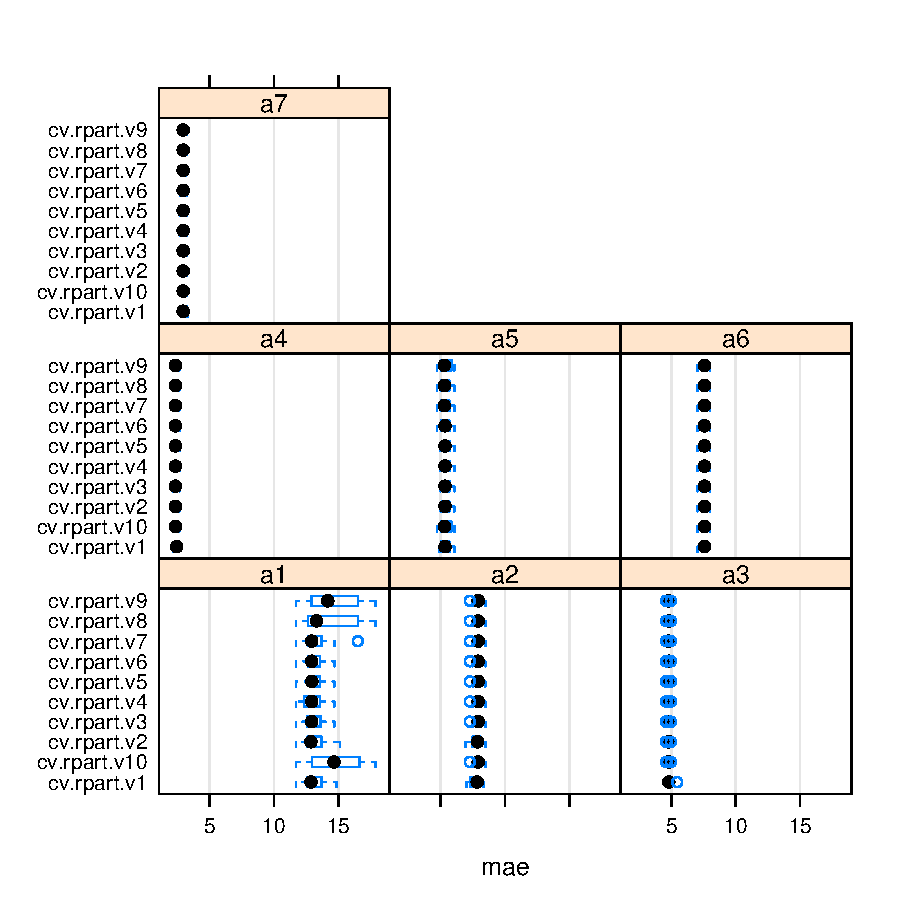
\includegraphics{KevinZollicoffer_Assignment2-007}

Getting best scores
\begin{Schunk}
\begin{Sinput}
> bs <- bestScores(res.all)
> bs
\end{Sinput}
\begin{Soutput}
$a1
         system    score
mae cv.rpart.v4 13.00495

$a2
         system   score
mae cv.rpart.v1 7.75812

$a3
         system    score
mae cv.rpart.v2 4.796588

$a4
         system    score
mae cv.rpart.v2 2.356468

$a5
         system    score
mae cv.rpart.v7 5.396761

$a6
         system    score
mae cv.rpart.v1 7.479273

$a7
         system   score
mae cv.rpart.v2 2.96584
\end{Soutput}
\end{Schunk}

Plotting best variants of models for the given algae

\begin{Schunk}
\begin{Sinput}
> # Subset by name not exact?
> res.all.v1 <- subset(res.all, vars='cv.rpart.v1')
> plot(res.all.v1)
\end{Sinput}
\end{Schunk}
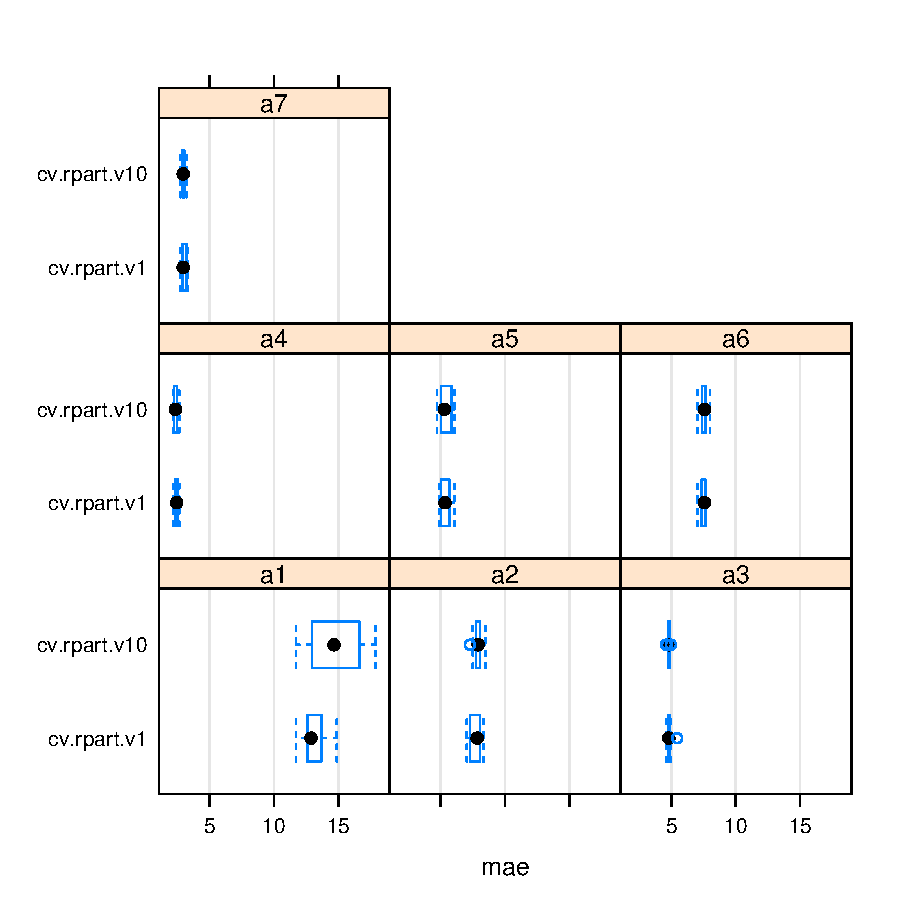
\includegraphics{KevinZollicoffer_Assignment2-009}

\begin{Schunk}
\begin{Sinput}
> # Subset by name not exact?
> res.all.v2 <- subset(res.all, vars='cv.rpart.v2')
> plot(res.all.v2)
\end{Sinput}
\end{Schunk}
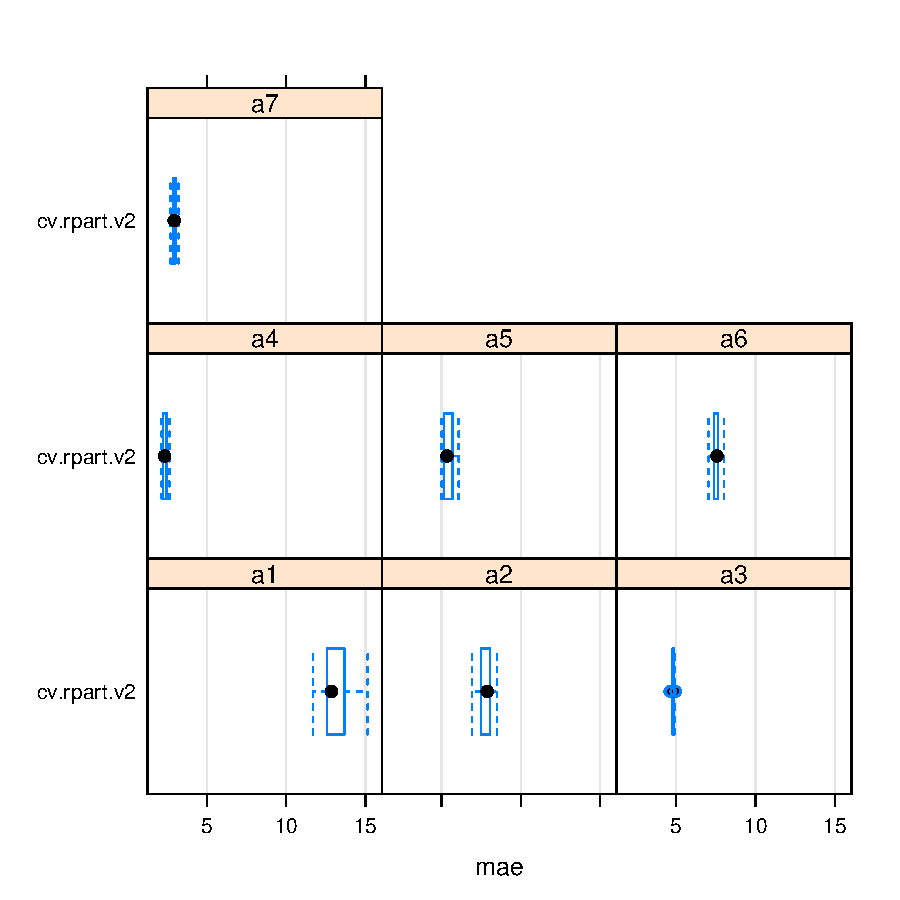
\includegraphics{KevinZollicoffer_Assignment2-010}

\begin{Schunk}
\begin{Sinput}
> # Subset by name not exact?
> res.all.v5 <- subset(res.all, vars='cv.rpart.v5')
> plot(res.all.v5)
\end{Sinput}
\end{Schunk}
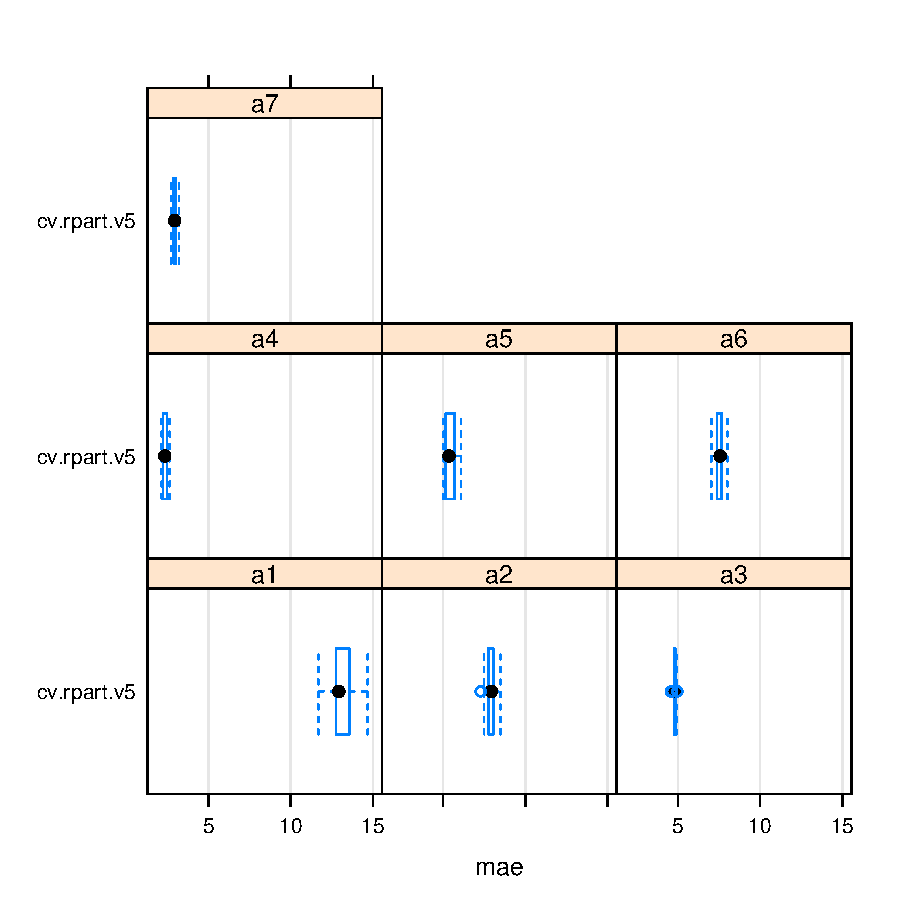
\includegraphics{KevinZollicoffer_Assignment2-011}
\end{document}
